\documentclass[12pt,letterpaper]{article}

\usepackage{amsmath, amsthm, amssymb, amsfonts}
\usepackage{graphicx}
\usepackage{bm}
\usepackage{natbib}

\theoremstyle{definition}
\newtheorem{dfn}{Definition}

\begin{document}

% The numbers below controls the amount of space between the following sections
\def\shiftdowna{0.32in}  % Adjust for balance
\def\shiftdownb{0.22in}  % Adjust for balance

% Set up the boiler plate at the top of the page

\begin{center}
\textbf{{\large Project Work Statement}}\\


% SPONSOR
\vspace \shiftdowna
\underline {Sponsor}\\ 
\vspace{5pt}
\textbf{{\large The GeoEye}}\\


% TITLE
\vspace \shiftdowna
\textbf{{\large Extracting Features from Ground-Track Images}}


% STUDENTS
\vspace{0.35in}
\vspace \shiftdownb
\underline {Participants} \\
\vspace{5pt}
\text{Nam Lee}, \texttt{nhlee@jhu.edu}

% SPONSORS
\vspace \shiftdownb
\underline {Potential Participants}\\
\vspace{5pt}
Youngser Park, \texttt{parky@jhu.edu} \\
\vspace{3pt}
\text{Mihn Tang}, \texttt{mtang10@jhu.edu} \\
\vspace{3pt}
\text{Glen Coppersmith}, \texttt{coppersmith@jhu.edu}

% DATE
\vspace \shiftdowna
Date: \today

\end{center}

\vfill  
%Fill page to force following note to bottom
\footnoterule
\noindent \small{Any apparent association of this work to The GeoEye is
fictional one, and the sole purpose of this work is a class exercise}

\newpage

\section{Background} 
GeoEye is a leading source of geospatial information and insight for decision
makers and analysts who need a clear understanding of our changing world to
protect lives, manage risk, and optimize resources. Each day, organizations in
defense and intelligence, public safety, critical infrastructure, energy, and
online media rely on GeoEye's imagery, tools, and expertise to support
important missions around the globe. Widely recognized as a pioneer in
high-resolution satellite imagery, GeoEye has evolved into a complete provider
of geospatial intelligence solutions. GeoEye's ability to collect, process,
and analyze massive amounts of geospatial data allows our customers to quickly
see precise changes on the ground and anticipate where events may occur in the
future.

\section{Problem Statement}
Consider the tracks reported in Figure \ref{fig:biketrack} extracted from an
``image'' taken from a satellite. 
\begin{figure}[h]
    \begin{center}
        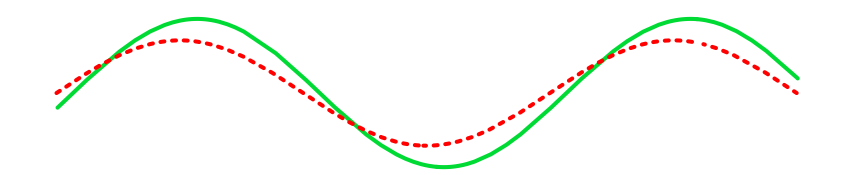
\includegraphics[width=\textwidth]{../images/sholmesbike.png}
    \end{center}
    \caption{A bicycle track}
    \label{fig:biketrack}
\end{figure}
To simplify our problem, we assume that the track is generated by a moving 
bicycle.  It is easy to see that the bicycle is swerving left and right,
but the general direction of the movement is not so obvious.  Nevertheless,
one can also identify the direction of the bicycle. 

The sponsor currently has a limited capability to make such inference from a
track of moving object from an image, and our task is to provide them with 
a reasonably large collection of such features and algorithms to detect them. 

\section{Approach}
Given a limited amount of our times, we will assume that extraction of 
tracts from an image is already completed.   
\section{Milestones}
We have the following major deadlines:
\begin{itemize}
    \item Work Statement due date, Sep 28, 2012,
    \item Midterm Presentation due date, Oct 12, 2012,
    \item Progress Report due date, Oct 26, 2012,
    \item Final Presentation due date, Nov 6, 2012,
    \item Final Report due date, Nov 30, 2012.
\end{itemize}

\section{Deliverable}
\subsection{From Team to Sponsor} % (fold)
The following outputs are expected from this project:
\begin{itemize}
    \item List of features of ground track useful for determining the
        target object and disambiguating the objects' moving direction 
    \item Algorithms for detecting the aforementioned features from images
    \item Numerical experiment results reporting performance of the developed algorithms
    \item R package with a complete set of documentations along with some test 
        codes that can be used to reproduce our numerical and simulation test
        results,
    \item Technical report and presentations summarizing the work. 
\end{itemize}

\subsection{From Sponsor to Team} % (fold)

In order for our project to be of successful one, we will need:
\begin{itemize}
    \item Images for training the numerical algorithms
    \item Computing resources
    \item Timely responses to inquiries, 
    \item Symposium attendance travel expenses.
\end{itemize}


%\newpage
%\bibliographystyle{plain}
%%\renewcommand\bibname{Selected Bibliography Including Cited Works}
%\nocite{*}
%\bibliography{biblio}

\end{document}
